\documentclass[conference]{IEEEtran}
\usepackage{cite}
\usepackage{amsmath,amssymb}
\usepackage{graphicx}
\usepackage{booktabs}
\usepackage{url}
\usepackage[hidelinks]{hyperref}
\usepackage{microtype}
\graphicspath{{figs/}}

\begin{document}

\title{Criterion-Level Clinical Trial Eligibility Matching with a Fine-Tuned Small Transformer: KV-Cached, Tiled-Attention and Speculative Inference on a 6\,GB GPU}

\author{\IEEEauthorblockN{Abdullah Nasir}
\IEEEauthorblockA{\textit{Department of Computer Science} \\
\textit{FAST National University of Computer and Emerging Sciences (FAST-NUCES), Islamabad} \\
23I-0726 --- i230726@isb.nu.edu.pk}}

\maketitle

\begin{abstract}
We study whether a small open-weight decoder-only Transformer can match patient descriptions to individual clinical-trial inclusion and exclusion criteria, cite the supporting patient sentences, and run on a 6\,GB laptop GPU. Using only the TrialGPT Criterion Annotations dataset with a fixed patient-grouped 37/8/8 split, we fine-tune Qwen2.5-1.5B-Instruct with LoRA to output an eligibility label from eight expert categories together with evidence sentence IDs. In addition to the supervised model we implement, test and benchmark three inference mechanisms from scratch: key/value-cached greedy decoding, exact tiled attention with online softmax, and greedy speculative decoding with a fine-tuned 0.5B draft model, and we integrate them in a browser application that produces an exportable screening report. We report before/after fine-tuning results, per-class and per-criterion-type metrics, evidence retrieval scores, an error analysis, and measured latency, throughput and memory, including cases where the optimisation does not help. The system is an educational screening prototype and not a clinical enrollment decision tool.
\end{abstract}

\begin{IEEEkeywords}
clinical trial matching, large language models, LoRA, KV cache, online softmax attention, speculative decoding
\end{IEEEkeywords}

\section{Introduction}
Recruiting patients for clinical trials requires reading a patient description and checking it against every inclusion and exclusion criterion of a trial. Each criterion is a short free-text statement (e.g., ``history of bleeding disorder''), and for most criteria the patient note simply does not contain enough information to decide. TrialGPT~\cite{jin2024trialgpt} showed that large language models can perform this \emph{criterion-level} matching and justify each decision with sentences from the patient record, but it relies on a large proprietary model (GPT-4).

This project asks a more modest question: \emph{how far can a small, locally executable open-weight Transformer (1.5\,B parameters, a 6\,GB laptop GPU) go on the same task when it is fine-tuned on the publicly released expert annotations?} In addition, the system must expose the inference machinery of a decoder-only Transformer: an explicit key/value (KV) cache, an exact tiled attention with online softmax, and greedy speculative decoding. The contributions of this report are:
\begin{enumerate}
\item a fixed, patient-grouped evaluation protocol (37/8/8 patients, seed 42) with no leakage of GPT-4 outputs, and a before/after comparison of Qwen2.5-1.5B-Instruct~\cite{qwen2024qwen25} adapted with LoRA~\cite{hu2022lora};
\item a criterion-level classifier that preserves all expert categories (including \emph{not enough information} and \emph{not applicable}) and returns cited sentence IDs, evaluated with accuracy, macro-F1, per-class metrics, confusion matrices and evidence precision/recall/F1;
\item from-scratch implementations of cache-aware decoding, tiled online-softmax attention and cache-synchronised greedy speculative decoding, each verified against a reference and benchmarked honestly;
\item a browser application that integrates these components and exports a screening report.
\end{enumerate}
The system is an educational screening prototype, not a tool for clinical enrollment decisions.

\section{Related Work}
\textbf{Clinical trial matching.} TrialGPT~\cite{jin2024trialgpt} decomposes patient--trial matching into criterion-level classification, evidence sentence retrieval and trial-level ranking, and released expert annotations of 1015 patient--criterion pairs~\cite{ncbi2024trialgptdata}. We use only that annotated benchmark and treat the paper's GPT-4 predictions strictly as unusable for input or evaluation. The original system depends on API-served models; our work instead studies supervised adaptation of a small open-weight model.

\textbf{Transformers and efficient adaptation.} Decoder-only Transformers~\cite{vaswani2017attention} with rotary position embeddings~\cite{su2024roformer} are the basis of the Qwen2.5 family~\cite{qwen2024qwen25}, Llama~3.2~\cite{meta2024llama32}, Gemma~2~\cite{gemma2024gemma2} and Phi-3~\cite{abdin2024phi3}. Parameter-efficient adaptation such as LoRA~\cite{hu2022lora} trains low-rank updates of the weight matrices while the base model stays frozen, and QLoRA~\cite{dettmers2023qlora} additionally quantises the frozen weights to 4~bit. We evaluate plain LoRA on fp16 weights because the 1.5\,B model fits in 6\,GB, which avoids quantisation noise in the later numerical experiments.

\textbf{Efficient attention.} Standard attention materialises an $L\times L$ score matrix. Milakov and Gimelshein~\cite{milakov2018online} showed that the softmax normaliser can be computed in a single pass with a running maximum, and FlashAttention~\cite{dao2022flashattention} combines this online softmax with tiling so that the score matrix never leaves fast on-chip memory. We implement the algorithm in PyTorch for correctness, and compare it with PyTorch's fused scaled-dot-product-attention backend.

\textbf{Inference acceleration.} KV caching removes the redundant recomputation of past keys and values~\cite{pope2023efficiently}, but the cache grows linearly with sequence length and dominates serving memory, motivating systems such as PagedAttention~\cite{kwon2023pagedattention}. Speculative decoding~\cite{leviathan2023speculative,chen2023speculative} lets a cheap draft model propose several tokens that the large target model verifies in one forward pass; for greedy decoding the output is identical to the target's own greedy output. We implement the greedy variant with explicit cache synchronisation.

\section{Materials and Methods}

\subsection{Dataset and Fixed Split}
We use only the TrialGPT Criterion Annotations dataset~\cite{ncbi2024trialgptdata}: 1015 rows from 53 patients and 103 trials. Each row contains a patient note whose sentences are numbered from~0, a trial title, a criterion type (inclusion or exclusion), the criterion text, an expert eligibility label and the expert-selected evidence sentence IDs. Inclusion criteria use the labels \emph{included}, \emph{not included}, \emph{not enough information} (NEI) and \emph{not applicable} (N/A); exclusion criteria use \emph{excluded}, \emph{not excluded}, NEI and N/A. All eight categories are preserved. The dataset also contains GPT-4 explanations, sentences and eligibility predictions; these columns, together with the dataset's own \texttt{training} flag, are dropped in \texttt{data/prepare\_data.py} so they can never be used as input or leak into evaluation.

Following the assignment protocol, the sorted unique patient IDs are shuffled with \texttt{numpy.random.default\_rng(42)}; the first 37 patients form the training split, the next 8 the validation split and the remaining 8 the test split. This gives 603, 206 and 206 annotations. The script asserts that the three patient sets are disjoint and that every annotation of a patient lies in exactly one split; the manifest (\texttt{data/split\_manifest.json}) lists all patient IDs and counts. Hyperparameters and the final adapter were chosen on the validation split only; the test split was evaluated once at the end.

Two properties of the data shape the evaluation (Table~\ref{tab:data}). First, the label distribution is strongly skewed: \emph{not excluded} alone is 44\,\% of the test rows, and the test split contains no \emph{excluded} example at all. Second, 60\,\% of all rows (70\,\% of test rows) have an \emph{empty} expert evidence set, so the treatment of empty sets matters for the evidence metrics.

\begin{table}[t]
\caption{Number of annotations per split and label (inclusion / exclusion criteria).}
\label{tab:data}
\centering\footnotesize
\begin{tabular}{lrrr}
\hline
Label & Train & Val & Test \\
\hline
included & 88 & 35 & 27 \\
not included & 13 & 3 & 7 \\
excluded & 8 & 2 & 0 \\
not excluded & 292 & 101 & 91 \\
NEI (incl.\,/\,excl.) & 109\,/\,65 & 27\,/\,26 & 38\,/\,28 \\
N/A (incl.\,/\,excl.) & 5\,/\,23 & 1\,/\,11 & 3\,/\,12 \\
\hline
Total annotations & 603 & 206 & 206 \\
Patients & 37 & 8 & 8 \\
Rows with empty gold evidence & 349 & 116 & 145 \\
\hline
\end{tabular}
\end{table}

\subsection{Model Candidates and Selection}
The task needs a decoder-only model that is open-weight, runs locally, supports autoregressive decoding with a KV cache, and can be fine-tuned and benchmarked on a laptop GPU with 6\,GB of VRAM (RTX~4050). Table~\ref{tab:models} compares candidates; fp16 weight memory is $2\times$ the parameter count. Training additionally needs activations, LoRA parameters and optimizer states, so a model whose fp16 weights alone approach the VRAM size is not usable without 4-bit quantisation, which would also confound the numerical comparisons in Tasks~3--5.

\begin{table*}[t]
\caption{Open-weight decoder candidates. Parameter counts and context windows are from the model cards (Qwen values verified from the downloaded \texttt{config.json}). ``fp16'' is the weight memory only.}
\label{tab:models}
\centering\footnotesize
\begin{tabular}{lrrrllp{3.6cm}}
\hline
Model & Params & Context & fp16 & License & Fits 6\,GB LoRA? & Decision \\
\hline
Qwen2.5-0.5B-Instruct & 0.49\,B & 32\,768 & 1.0\,GB & Apache-2.0 & yes & \textbf{draft model} (same tokenizer as the 1.5B) \\
Qwen2.5-1.5B-Instruct & 1.54\,B & 32\,768 & 3.1\,GB & Apache-2.0 & yes (3.9\,GB peak) & \textbf{selected target} \\
Llama-3.2-1B-Instruct~\cite{meta2024llama32} & 1.24\,B & 131\,072 & 2.5\,GB & Llama 3.2 community & yes & not used: gated download, restrictive license, no smaller same-tokenizer draft \\
Gemma-2-2B-it~\cite{gemma2024gemma2} & 2.6\,B & 8\,192 & 5.2\,GB & Gemma terms & no (weights alone fill VRAM) & rejected: memory \\
Qwen2.5-3B-Instruct & 3.09\,B & 32\,768 & 6.2\,GB & Qwen research & no & rejected: memory, license \\
Phi-3-mini-4k~\cite{abdin2024phi3} & 3.8\,B & 4\,096 & 7.6\,GB & MIT & no & rejected: memory \\
\hline
\end{tabular}
\end{table*}

We selected \textbf{Qwen2.5-1.5B-Instruct}~\cite{qwen2024qwen25}: 28 Transformer layers, hidden size 1536, 12 query heads and 2 key/value heads (grouped-query attention, head size 128), SwiGLU feed-forward size 8960, rotary position embeddings ($\theta=10^6$), RMSNorm, tied input/output embeddings, a 151\,936-token BPE vocabulary and a 32\,768-token context window; 1\,543\,714\,304 parameters, Apache-2.0 license. Because only 2 KV heads are cached, the KV cache costs $2\cdot 28\cdot 2\cdot 128\cdot 2\,\text{B}=28\,672$\,B (28\,KiB) per token in fp16, so even the longest prompt (555 tokens) needs only 15.5\,MiB of cache. For speculative decoding we use \textbf{Qwen2.5-0.5B-Instruct} as draft (494\,032\,768 parameters, 24 layers, hidden size 896, 14 query heads, 2 KV heads); we verified programmatically that its vocabulary is identical to the target's, which is required for token-level verification. We did not train the other candidates, so the choice rests on the resource analysis above and not on an empirical comparison; we state this as a limitation.

\subsection{Input/Output Format and Tokenization}
Each example is rendered with the model's chat template. The user message contains the patient note with its sentence IDs, the criterion type, the criterion text and the list of allowed labels for that type; the system message states that the model may use only the note. The target answer is a one-line JSON object, e.g. \texttt{\{"label": "included", "evidence": [0, 2]\}}, followed by the end-of-turn token. Only the answer tokens contribute to the loss. A tolerant parser (\texttt{src/prompts.py}) extracts the label and sentence IDs; a label outside the allowed set for the criterion type, or an unparsable output, is counted as an \emph{invalid} prediction and is never silently mapped to a class. Cited IDs outside the note are discarded.

\textbf{Truncation.} Using the Qwen tokenizer, prompts have a mean of 272 tokens (training) and a maximum of 555 tokens; the answer averages 14 tokens (maximum 37). With a 1024-token cap, \emph{no example in any split is truncated}, so no patient evidence is lost (\texttt{results/token\_stats.json}).

\subsection{Fine-Tuning}
We fine-tune with LoRA~\cite{hu2022lora} on all seven linear projections of every layer (query, key, value, output, gate, up, down) with rank $r=16$, $\alpha=32$ and dropout 0.05, giving 18\,464\,768 trainable parameters (1.18\,\% of the model). The frozen base is kept in fp16, the LoRA weights in fp32, with fp16 autocast, gradient checkpointing and a gradient scaler. We use AdamW (no weight decay), peak learning rate $2\times10^{-4}$ with 5\,\% linear warm-up and cosine decay, gradient clipping at 1.0, micro-batch 4 with 4 accumulation steps (effective batch 16) and seed 42. The objective is next-token cross-entropy on the answer tokens. A 152k-way logit tensor for a whole batch does not fit in 6\,GB, so the training code runs the Transformer body, selects only the hidden states that predict answer tokens (about 14 per example) and applies the output layer there; this yields exactly the same loss with a small fraction of the memory (our first attempt with full logits stalled at 5.9\,GiB). The validation loss is computed after every epoch and the adapter with the lowest validation loss is kept. As a second configuration we add \emph{class-balanced oversampling} of the training split: every (type, label) group is repeated $\text{round}\bigl(\sqrt{n_\text{max}/n}\bigr)$ times to counter the dominance of \emph{not excluded} and NEI.

\subsection{KV-Cached Autoregressive Decoding}
\label{sec:kvmethod}
Two greedy decoders are implemented around the same weights (\texttt{src/kv\_decode.py}). The \emph{reference} decoder re-runs the model on the whole sequence for every generated token. The \emph{cache-aware} decoder prefills the prompt once while a \texttt{DynamicCache} that we create collects the keys and values of all 28 layers, and then feeds only the newest token at each step. We pass the cache, the absolute \texttt{position\_ids}/\texttt{cache\_position} (equal to the number of cached tokens) and an all-ones attention mask of length $\text{cache}+1$ ourselves:
\begin{itemize}
\item \emph{Positional handling.} Qwen2.5 uses rotary embeddings, which rotate queries and keys by an angle proportional to their absolute position. Keys are stored \emph{after} rotation, so a cached key never needs to be recomputed, but the new token must be rotated with its true position; giving it position~0 would silently corrupt the output.
\item \emph{Masking.} During prefill the model applies the lower-triangular causal mask. In a decode step the single query is the last position, so it may attend to every cached key and no explicit triangular mask is required; the attention mask only marks valid (non-padding) positions.
\item \emph{Cache growth.} Each step appends one key and one value vector per layer and KV head, so the cache grows linearly by 28\,KiB per token for this model and decode attention costs $O(n)$ per step instead of re-processing the whole prefix ($O(n)$ tokens through all layers).
\item \emph{Numerical differences.} Cached and uncached passes sum the same terms in a different order and with different matrix shapes (a $1\times n$ product versus an $n\times n$ product), so logits agree only up to floating-point rounding. A greedy token can change only if the two best logits are closer than this rounding error; we measure the logit differences and top-1/top-2 margins in Section~\ref{sec:kvres}.
\end{itemize}

\subsection{Tiled Attention with Online Softmax}
\label{sec:attmethod}
For queries $Q\in\mathbb{R}^{L_q\times d}$ and keys/values $K,V\in\mathbb{R}^{L_k\times d}$ the reference implementation computes $S=QK^\top/\sqrt d$, applies the causal mask, subtracts the row maximum for numerical stability and returns $\mathrm{softmax}(S)V$. For $L_q<L_k$ (decoding with a cache) causality is bottom-right aligned: query $i$ may attend to key $j$ iff $j\le i+(L_k-L_q)$.

The tiled version (\texttt{src/attention.py}) processes $Q$ in blocks of $B_q$ rows and sweeps over blocks of $B_k$ keys while keeping, for every query row, a running maximum $m$, a running normaliser $\ell$ and a running unnormalised output $o$. For a new score tile $S_t$ with row maximum $\tilde m$:
\begin{align}
m' &= \max(m,\tilde m), \quad \alpha=e^{m-m'}, \quad P=e^{S_t-m'},\\
\ell' &= \alpha\,\ell+\textstyle\sum_j P_{\cdot j}, \qquad o' = \alpha\,o + P\,V_t,
\end{align}
and the final output is $o/\ell$. This equals exact softmax attention (no approximation) while only a $B_q\times B_k$ tile of scores exists at any time; accumulators are kept in float32. Key blocks that lie entirely above the causal diagonal are skipped, and rows that have seen only masked keys keep $m=-\infty$ and are guarded against $\infty-\infty$.

\subsection{Greedy Speculative Decoding}
\label{sec:specmethod}
The implementation (\texttt{src/speculative.py}) maintains the invariant that both models' caches contain the first $c$ tokens of the sequence and that the last token \texttt{last} is not yet cached. One round consists of:
\begin{enumerate}
\item \textbf{Draft.} The draft model greedily proposes $k$ tokens $d_1..d_k$ one at a time, extending its own cache.
\item \textbf{Verify.} The target processes $[\texttt{last},d_1,\dots,d_k]$ in \emph{one} forward pass and produces its greedy choice $p_i$ after each position.
\item \textbf{Accept.} Let $m$ be the length of the longest prefix with $d_{i+1}=p_i$. We emit $d_1..d_m$ and then $p_m$: the target's \emph{correction} for the first rejected token if $m<k$, or a free \emph{bonus} token if $m=k$. Each round therefore yields between 1 and $k+1$ tokens, all of them target-greedy tokens.
\item \textbf{Synchronise.} The target cache holds $c+k+1$ positions but only the first $c+m+1$ are valid, so it is cropped to $c+m+1$; the draft cache is cropped likewise, and if $m=k$ the draft first consumes $d_k$, which it proposed but never fed. The new \texttt{last} is $p_m$.
\end{enumerate}
We report the acceptance rate (accepted draft tokens / drafted tokens), the mean number of tokens per target forward pass, wall-clock time, throughput and peak memory, and verify token equality with plain cached greedy decoding and with the Hugging Face assisted-generation API (used only as a reference test).

\subsection{Application Workflow}
The Gradio application (\texttt{app/app.py}) takes a patient note (numbered sentences are kept; free text is split into sentences automatically), an optional trial title, and inclusion and exclusion criteria (one per line). Inputs are validated (empty or too short note, no criteria, more than 30 criteria, overlong criteria, notes above 1500 tokens) and errors are shown instead of crashing. The user selects the inference mode (no cache, KV cache or speculative decoding with draft length $k$); for each criterion the model returns a label and sentence IDs, and the application shows the label, the cited IDs, the exact sentence text and a template explanation that quotes only the cited sentences (for NEI it states that the note does not settle the question). The trial-level outcome is an explicit rule-based aggregation, not a learned or ground-truth label: any \emph{not included} or \emph{excluded} criterion gives ``likely not eligible''; otherwise any NEI or invalid criterion gives ``undetermined''; otherwise ``likely eligible''. A live benchmark tab runs the three decoders on the user's input, and the report (HTML) records the model, adapter, decoding mode and timestamp. A prominent notice states that the system is an educational prototype, not a clinical enrollment decision.

\section{Experimental Setup and Metrics}
\textbf{Hardware and software.} All experiments ran on a single laptop with an NVIDIA GeForce RTX~4050 Laptop GPU (6\,GB VRAM, Windows~11), Python~3.11, PyTorch~2.5.1 (CUDA~12.1), Transformers~4.49.0~	te{wolf2020transformers}, PEFT~0.14.0 and Gradio~5.12.0 (pinned in \texttt{requirements.txt}). No paid GPU or API was used. Models are executed in fp16 unless stated otherwise.

\textbf{Decoding settings for comparisons.} Every accuracy comparison (zero-shot base model, fine-tuned model) uses the same prompts, the same examples, greedy decoding (no sampling), at most 48 new tokens, fp16 and left-padded batches of 8. Zero-shot means the \emph{same} Qwen2.5-1.5B-Instruct weights and the \emph{same} prompt with no adapter.

\textbf{Classification metrics.} We report accuracy, macro-F1, and per-class precision, recall and F1 with support, as well as confusion matrices, overall and separately for inclusion and exclusion criteria (label sets differ, so the two types are evaluated against their own four labels). Invalid outputs count as errors and are placed in an extra ``invalid'' column. Macro-F1 averages over classes that occur in the gold labels or the predictions of the evaluated slice; classes with neither gold nor predicted examples are skipped and are never counted as zero. Because some classes have very few test examples (Table~\ref{tab:data}), per-class scores are noisy and we always show supports.

\textbf{Evidence metrics.} For every row we compare the set of cited sentence IDs to the expert set. Micro scores pool true/false positives and false negatives over rows; macro scores average per-row precision, recall and F1. Empty sets are handled explicitly: if both gold and prediction are empty the row scores 1/1/1; if only the gold is empty a non-empty prediction scores precision 0, recall 1, F1 0; if only the prediction is empty precision is 1, recall 0 and F1 0. Since 60\,\% of the rows have empty gold evidence, we report evidence metrics on \emph{all rows} and on \emph{rows with non-empty gold evidence only}.

\textbf{Inference benchmarks.} Latency is measured with \texttt{time.perf\_counter} after \texttt{torch.cuda.synchronize()}, with one warm-up run before the timed repeats and the median reported; ``prefill'' is the time to the first generated token, ``decode'' the time for the remaining tokens, throughput is generated tokens per second, and peak memory is \texttt{torch.cuda.max\_memory\_allocated}. Because prompt lengths in the dataset are short (at most 555 tokens), length sweeps use real clinical text repeated to controlled lengths. Attention benchmarks use 12 heads of size 64 in fp16 with causal masking.

\section{Results and Discussion}

\subsection{Design Decisions, Rejected Alternatives and Observed Difficulties}
Table~\ref{tab:decisions} collects the main technical decisions, the alternatives that were considered or rejected, and the evidence that supported the final choice; the experimental evidence for each row is discussed in the subsections that follow.

\begin{table*}[t]
\caption{Design decisions, alternatives and evidence. ``Estimated'' values are back-of-the-envelope figures (about 16 bytes per parameter for mixed-precision AdamW), not measurements.}
\label{tab:decisions}
\centering\footnotesize
\begin{tabular}{p{2.3cm}p{3.5cm}p{4.6cm}p{5.6cm}}
\hline
Decision & Alternatives & Evidence / difficulty & Outcome \\
\hline
Base model & Llama-3.2-1B, Gemma-2-2B, Qwen2.5-3B, Phi-3-mini (Table~\ref{tab:models}) & Weights of the 2--4\,B models alone fill or exceed 6\,GB; Llama is gated and under a restrictive license & Qwen2.5-1.5B (Apache-2.0, 3.9\,GiB peak for training); only this model was trained. \\
Adaptation method & Full fine-tuning; QLoRA 4-bit & Full fine-tuning needs an estimated 25\,GB; QLoRA was unnecessary and would add quantisation noise to the numerical comparisons & LoRA $r=16$ on all linear layers over an fp16 base. \\
Loss computation & Logits over all positions & First attempt stalled at 5.9\,GiB (no progress after 4\,min) because of the 152k-way vocabulary & Output layer applied only at answer positions: 3.9\,GiB, 16\,s per step, same loss. \\
Label imbalance & Plain training; class-weighted or focal loss (not tried) & Plain run answered \emph{not excluded} for 139 of 140 validation exclusion rows (macro-F1 0.467) & Rare-label oversampling: validation macro-F1 0.534, exclusion macro-F1 0.377 $\rightarrow$ 0.567. \\
Output format & Classification head; free-text rationale & A head cannot return sentence IDs jointly and would not exercise autoregressive decoding; free text is hard to evaluate and may hallucinate & Single-line JSON (label, IDs); 0 invalid outputs on validation and test. \\
Number of epochs & 3 epochs & Validation loss was lowest after epoch 2 (0.1333) and rose slightly in epoch 3 (0.1358) & Best-validation-loss checkpoint; balanced run limited to 2 epochs. \\
Precision for cache tests & fp16 only & fp16 diverged from the reference in two of five settings; exact logit ties found & Same tests in fp32 on the 0.5\,B model: identical at all five settings (1.5\,B in fp32 does not fit). \\
Draft model & Untuned 0.5B draft & Untuned draft: acceptance 0.62 versus 0.90 ($k=4$), Table~\ref{tab:draftcmp} & Draft trained with the same recipe (11\,min). \\
Attention tile size & $64\times64$ versus $256\times256$ & 64: 7\,MiB but 34$\times$ slower than the dense reference; 256: 20\,MiB and 2$\times$ slower & Both reported; neither beats the fused kernel. \\
Engineering issues & -- & Large downloads stalled on this network; Gradio~5.12 failed to start with newer \texttt{pydantic} (reported as ``localhost not accessible'') & Resumable \texttt{curl} downloads; \texttt{pydantic} pinned to 2.10.6. \\
\hline
\end{tabular}
\end{table*}

\subsection{Fine-Tuning and Model Selection}
Table~\ref{tab:train} summarises the three training runs and Fig.~\ref{fig:train} shows their curves. Starting from the same frozen weights, the answer-token validation loss of the 1.5\,B model drops from 0.658 to 0.13--0.15 within the first epoch, and the zero-shot model that already produces valid JSON in 100\,\% of the cases is turned from a nearly useless classifier (validation accuracy 0.068, macro-F1 0.081) into a usable one (0.728 / 0.467). The first run (3 epochs, rank 16) reaches its best validation loss after epoch 2 (0.1333) and rises slightly in epoch 3 (0.1358), a mild sign of overfitting on 603 examples; the checkpoint with the lowest validation loss is kept.

Its validation confusion pattern revealed a structural problem: for exclusion criteria the model answered \emph{not excluded} for 139 of 140 rows and never predicted NEI or N/A, i.e.\ it had learned the majority class (101 of 140 gold labels). The second run therefore oversamples rare labels in the training split (Section~\ref{sec:methods}). It has almost the same validation loss (0.1324) but a clearly better macro-F1 (0.534 versus 0.467), because exclusion macro-F1 rises from 0.377 to 0.567 while overall accuracy is almost unchanged (0.733 versus 0.728). The selection between the two runs was made on the validation split only; the balanced run is the \emph{final adapter}. Loss alone could not have made this choice, which is why macro-F1 on the validation set was used. The 0.5\,B draft model was trained with the identical recipe in 11 minutes and 1.46\,GiB of GPU memory (validation loss 0.486 $\rightarrow$ 0.154).

\begin{table*}[t]
\caption{Training runs (LoRA rank 16, learning rate $2\times10^{-4}$, effective batch 16, seed 42, RTX 4050). Validation metrics are criterion-level on the 206 validation rows; ``val.\ loss'' is the answer-token cross-entropy of the selected checkpoint.}
\label{tab:train}
\centering\footnotesize
\begin{tabular}{llrrrrrrr}
\hline
Run & Model & Train rows $\times$ epochs & Val.\ loss before $\rightarrow$ after & Val.\ acc. & Val.\ macro-F1 & Time & Peak GPU \\
\hline
Zero-shot (no training) & Qwen2.5-1.5B & -- & 0.658 & 0.068 & 0.081 & -- & -- \\
LoRA, plain & Qwen2.5-1.5B & $603\times3$ & 0.658 $\rightarrow$ 0.1333 & 0.728 & 0.467 & 35.3 min & 3.88 GiB \\
LoRA, class-balanced (\textbf{final}) & Qwen2.5-1.5B & $823\times2$ & 0.658 $\rightarrow$ 0.1324 & \textbf{0.733} & \textbf{0.534} & 30.9 min & 3.88 GiB \\
LoRA, class-balanced (draft) & Qwen2.5-0.5B & $823\times2$ & 0.486 $\rightarrow$ 0.1536 & -- & -- & 11.0 min & 1.46 GiB \\
\hline
\end{tabular}
\end{table*}

\begin{figure}[t]
\centering
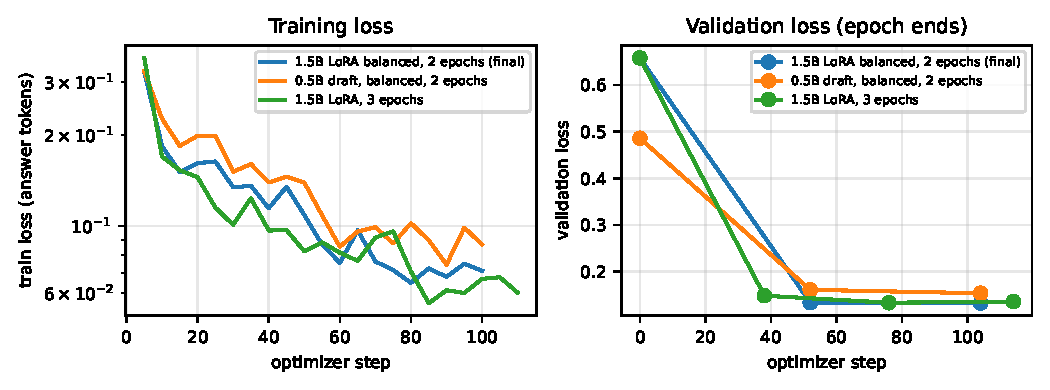
\includegraphics[width=\columnwidth]{training_curves}
\caption{Left: training loss on answer tokens (log scale, logged every 5 optimizer steps). Right: validation loss at epoch ends; step~0 is the untrained model. The three runs converge to a similar validation loss; the draft model (0.5\,B) ends higher than the 1.5\,B model.}
\label{fig:train}
\end{figure}

\subsection{Criterion-Level Eligibility on the Held-Out Test Split}
All numbers in this subsection come from the single evaluation of the test split (8 patients, 206 criteria) after the final adapter had been chosen on validation. Table~\ref{tab:main} compares three systems on identical examples with identical decoding: a trivial \emph{majority-per-type} predictor (the most frequent training label for each criterion type), the zero-shot base model, and the fine-tuned model.

\begin{table*}[t]
\caption{Held-out test results (206 criteria, 8 patients). Accuracy / macro-F1 are computed overall and separately for inclusion (75 rows) and exclusion (131 rows) criteria; evidence micro-F1 is reported over all rows and over the 61 rows with non-empty expert evidence. Macro-F1 averages over the classes present in gold or predictions (no \emph{excluded} example exists in the test split). Brackets: 95\,\% patient-level bootstrap interval (2000 resamples) for the fine-tuned model and the zero-shot baseline.}
\label{tab:main}
\centering\footnotesize
\begin{tabular}{lcccccc}
\hline
System & Overall acc.\,/\,F1 & Inclusion acc.\,/\,F1 & Exclusion acc.\,/\,F1 & Invalid & Evid.\ F1 (all) & Evid.\ F1 (gold-only) \\
\hline
Majority per type & 0.626 / 0.272 & 0.507 / 0.168 & 0.695 / 0.273 & 0 & 0.000 & 0.000 \\
Zero-shot Qwen2.5-1.5B & 0.058 / 0.084 & 0.120 / 0.114 & 0.023 / 0.040 & 0 & 0.122 & 0.398 \\
\hspace{3mm}95\,\% interval & [.031,.099] / [.042,.125] & -- / [.047,.180] & -- / [.000,.083] & & [.061,.203] & -- \\
\textbf{Fine-tuned (LoRA, balanced)} & \textbf{0.718 / 0.604} & \textbf{0.787 / 0.579} & 0.679 / \textbf{0.500} & 0 & \textbf{0.531} & \textbf{0.636} \\
\hspace{3mm}95\,\% interval & [.602,.803] / [.491,.675] & -- / [.415,.720] & -- / [.424,.617] & & [.456,.642] & -- \\
\hline
\end{tabular}
\end{table*}

Fine-tuning improves every headline metric: accuracy rises from 0.058 to 0.718, macro-F1 from 0.084 to 0.604, and the intervals of the two systems do not overlap, although they are wide because only eight patients are tested. Against the majority baseline the picture is more nuanced and should not be glossed over: on \emph{inclusion} criteria the model is clearly better (0.787 versus 0.507 accuracy), but on \emph{exclusion} criteria its accuracy (0.679) is slightly \emph{below} the always-\emph{not excluded} predictor (0.695); it only wins on macro-F1 (0.500 versus 0.273) because it recognises some \emph{not applicable} cases. The zero-shot model's behaviour is also informative: it labels 124 of 131 exclusion criteria \emph{excluded}, apparently reading ``the criterion describes something that applies'' as ``exclude'', and it never says NEI; most of the gain from fine-tuning is therefore learning the task's label semantics.

\begin{table}[t]
\caption{Per-class results of the fine-tuned model on the test split (supports are gold counts); F1 of the zero-shot model in the last column. ``--'': no gold and no fine-tuned prediction.}
\label{tab:perclass}
\centering\footnotesize
\begin{tabular}{llrrrrr}
\hline
Type & Class & P & R & F1 & Supp. & Zero-shot F1 \\
\hline
incl. & included & 0.96 & 0.81 & 0.88 & 27 & 0.36 \\
incl. & not included & 0.50 & 0.14 & 0.22 & 7 & 0.00 \\
incl. & NEI & 0.73 & 0.92 & 0.81 & 38 & 0.00 \\
incl. & N/A & 0.50 & 0.33 & 0.40 & 3 & 0.09 \\
excl. & excluded & -- & -- & -- & 0 & 0.00 \\
excl. & not excluded & 0.72 & 0.89 & 0.79 & 91 & 0.04 \\
excl. & NEI & 0.25 & 0.11 & 0.15 & 28 & 0.00 \\
excl. & N/A & 0.83 & 0.42 & 0.56 & 12 & 0.12 \\
\hline
\end{tabular}
\end{table}

Table~\ref{tab:perclass} and the confusion matrices in Figs.~\ref{fig:confb} and~\ref{fig:conff} show where the remaining errors lie. For inclusion criteria, \emph{included} is predicted with high precision (0.96), and the dominant confusion is the model answering NEI for 5 included and 6 not-included cases, so it is conservative about asserting a decision. For exclusion criteria the behaviour is the opposite: 25 of 28 NEI rows are labelled \emph{not excluded} (recall 0.11), i.e.\ the model treats ``not mentioned'' as ``not a problem'', exactly the inference the task warns against. \emph{Not applicable} has high precision but low recall (0.42 for exclusion; 7 of 12 are called \emph{not excluded}). The rarest classes (\emph{not included}: 7 rows, inclusion N/A: 3 rows) have F1 values that rest on a handful of examples and should be read as indicative only. Because the test split contains no \emph{excluded} example, the ability to detect an excluded patient is not measured at all by this evaluation, a limitation of the fixed split rather than of the model (the validation split has only two such examples).

\begin{figure}[t]
\centering
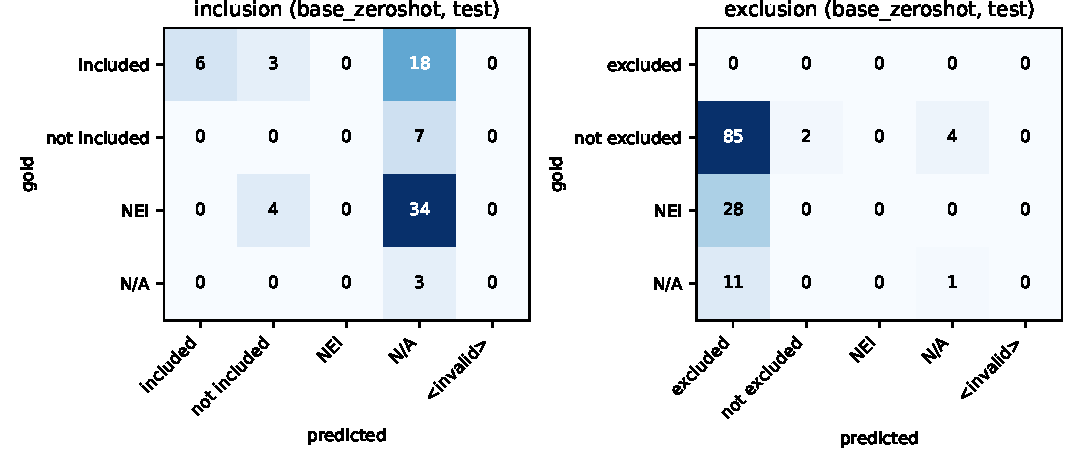
\includegraphics[width=\columnwidth]{confusion_base_zeroshot_test}
\caption{Confusion matrices of the zero-shot base model on the test split (rows: gold, columns: predicted; NEI = not enough information, N/A = not applicable). The base model sends almost all exclusion criteria to \emph{excluded} and never predicts NEI.}
\label{fig:confb}
\end{figure}

\begin{figure}[t]
\centering
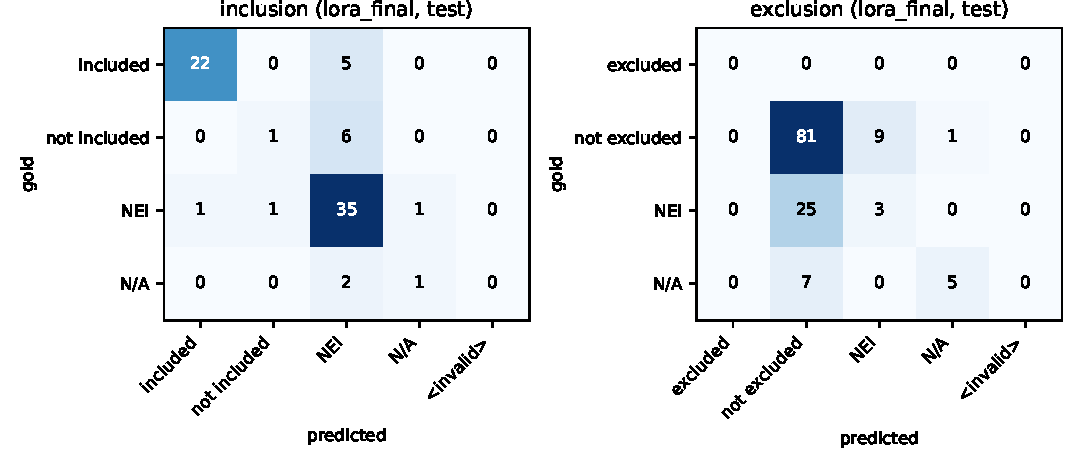
\includegraphics[width=\columnwidth]{confusion_lora_final_test}
\caption{Confusion matrices of the fine-tuned model on the test split. Inclusion (left) is concentrated on the diagonal with a tendency toward NEI; exclusion (right) is dominated by \emph{not excluded}, with 25 NEI rows absorbed into that class.}
\label{fig:conff}
\end{figure}

\subsection{Evidence Sentence Retrieval}
Table~\ref{tab:evidence} reports sentence-level evidence scores using the empty-set rules of Section~\ref{sec:setup}. Since 145 of the 206 test rows have no expert evidence, an annotator-style ``cite nothing'' answer is usually right, and overall scores must be read together with the second block that only counts the 61 rows with expert evidence. The fine-tuned model reaches a micro-F1 of 0.531 over all rows (zero-shot: 0.122) and 0.636 over rows with gold evidence (zero-shot: 0.398), with precision 0.683 and recall 0.596 on the latter. It cites nothing for 143 rows (experts: 145) and for both-empty rows it is right 125 times, so its per-row (macro) scores are high (0.782) mostly because of such rows; the micro scores are more informative. Evidence is much better localised for inclusion (micro-F1 0.618) than for exclusion criteria (0.305) over all rows. In 18 of the 61 evidence rows the model cites nothing, which accounts for most of the missing recall.

\begin{table}[t]
\caption{Evidence-sentence retrieval on the test split. ``Micro'' pools sentence counts over rows; ``macro'' averages per-row scores (empty-versus-empty rows count as 1).}
\label{tab:evidence}
\centering\footnotesize
\begin{tabular}{lcccccc}
\hline
 & \multicolumn{3}{c}{Micro} & \multicolumn{3}{c}{Macro} \\
System / rows & P & R & F1 & P & R & F1 \\
\hline
Zero-shot, all (206) & 0.073 & 0.372 & 0.122 & 0.378 & 0.773 & 0.212 \\
Zero-shot, gold-evidence (61) & 0.427 & 0.372 & 0.398 & 0.753 & 0.234 & 0.191 \\
Fine-tuned, all (206) & 0.479 & 0.596 & 0.531 & 0.869 & 0.893 & 0.782 \\
Fine-tuned, gold-evidence (61) & 0.683 & 0.596 & 0.636 & 0.886 & 0.638 & 0.592 \\
\hline
\end{tabular}
\end{table}

\subsection{Error Analysis}
Of 206 test predictions, 58 have a wrong label (\texttt{results/error\_analysis\_final.md} contains the full notes of every case below). The most frequent confusion is gold NEI predicted as \emph{not excluded} (25 cases, 43\,\% of all errors); 42 of the 58 wrong predictions cite no evidence at all, and 27 of the 66 gold-NEI rows received a decisive label. Table~\ref{tab:errors} lists twelve distinct cases that illustrate the failure modes.

\begin{table*}[t]
\caption{Twelve distinct test errors (annotation IDs refer to the dataset; full note text and quoted sentences are in the repository). NEI = not enough information, N/A = not applicable.}
\label{tab:errors}
\centering\footnotesize
\begin{tabular}{rlp{4.1cm}lp{6.8cm}}
\hline
\# & Ann. & Criterion (type) & Gold $\rightarrow$ predicted & Explanation of the failure \\
\hline
1 & 174 & Previous axillary surgery (excl.) & NEI $\rightarrow$ not excluded & Note never mentions surgical history; absence read as proof of eligibility. \\
2 & 193 & Patients were moribund (excl.) & NEI $\rightarrow$ not excluded & Pale, tachycardic, BP 80/60 suggest severity but cannot establish it; model cited nothing and ignored the cues. \\
3 & 389 & Severe renal impairment, GFR $<$ 50\,\% (excl.) & NEI $\rightarrow$ not excluded & Proteinuria and RBC casts hint at kidney disease but no GFR is given; hints ignored. \\
4 & 325 & ``Genetic patients'' (incl.) & NEI $\rightarrow$ not included & Vague criterion; model cited the CVID sentence as if it disproved a genetic cause (unsupported). \\
5 & 185 & Diagnosed with shock or ARDS (incl.) & included $\rightarrow$ NEI & ``Shock'' is never written; it is implied by BP 80/60, pallor, tachycardia. Needs inference, not keyword matching. \\
6 & 188 & Vasopressors to keep SBP $\ge$ 90 (incl.) & not incl. $\rightarrow$ NEI & Gold label depends on a judgement call (low BP without any drug mentioned); model hedges. \\
7 & 162 & Open abdominal aortic aneurysm repair (incl.) & not incl. $\rightarrow$ NEI & Patient has a femoral access-site problem; asserting a negative inclusion is rare for the model (recall 1/7). \\
8 & 745 & Female patients with birth control (incl.) & N/A $\rightarrow$ NEI & Patient is a 5-year-old boy; applicability hinges on the single word ``boy'' in sentence~0. \\
9 & 743 & Daily access to e-mail (incl.) & NEI $\rightarrow$ N/A & Same boy; NEI versus N/A is a subjective boundary. \\
10 & 422 & If female, using birth control (incl.) & N/A $\rightarrow$ NEI & Experts and model cite the same sentence (``no sexual partners'') but decide differently. \\
11 & 186 & Heart rate $\ge$ 90/min (incl.) & included $\rightarrow$ included & Correct label but cites the blood-pressure sentence instead of ``tachycardic''; explanation would not support the decision. \\
12 & 179 & Prior central venous catheterization (excl.) & not excl. $\rightarrow$ not excl. & Correct label, but the related arterial-catheterization sentence is not cited (under-citation). \\
\hline
\end{tabular}
\end{table*}

Three patterns emerge. (i)~\emph{False certainty on missing information} (cases 1--4): the model prefers the majority label over admitting that the note is silent, particularly for exclusion criteria, which are overwhelmingly \emph{not excluded} in the training data (292 of 388 exclusion rows). (ii)~\emph{Implicit evidence} (cases 5--7): when a criterion requires clinical inference rather than lexical overlap, the 1.5\,B model is unreliable. (iii)~\emph{Label-boundary ambiguity} (cases 6, 8--10): the NEI/N/A/negative boundaries are subjective, so part of the error is annotation noise. Cases 11 and 12 show that a correct label can still come with an incomplete or wrong citation, which matters for a screening tool whose explanations are supposed to be traceable.

\subsection{KV-Cached Decoding}
\label{sec:kvres}
\textbf{Correctness.} Table~\ref{tab:kvcorr} compares the cache-aware decoder of Section~\ref{sec:kvmethod} with the uncached reference under greedy decoding for five prompt/output length combinations. In fp32 (the 0.5\,B model; the 1.5\,B model does not fit in fp32 in 6\,GB) the two decoders produce \emph{identical} tokens at all five settings, and the final cache length equals prompt length plus generated tokens minus one in every case, as the invariant (the last generated token has not been fed back) requires. With the fine-tuned 1.5\,B model in fp16 three of five settings are identical, but two diverge (at 0-based generated-token index 44 for 256+128 and 25 for 512+64); all later differences follow from that first one because the contexts differ afterwards.

\begin{table}[t]
\caption{Token equality of the KV-cached decoder versus the uncached reference (greedy). ``First diff.'' is the index of the first differing generated token; the final cache length always equals prompt + new tokens $-1$ (not shown, matched in all rows).}
\label{tab:kvcorr}
\centering\footnotesize
\begin{tabular}{llrrcr}
\hline
Model & Precision & Prompt & New & Identical & First diff. \\
\hline
1.5B fine-tuned & fp16 & 32 & 16 & yes & -- \\
1.5B fine-tuned & fp16 & 128 & 64 & yes & -- \\
1.5B fine-tuned & fp16 & 256 & 128 & \textbf{no} & 44 \\
1.5B fine-tuned & fp16 & 512 & 64 & \textbf{no} & 25 \\
1.5B fine-tuned & fp16 & 700 & 32 & yes & -- \\
0.5B base & fp32 & 32 & 16 & yes & -- \\
0.5B base & fp32 & 128 & 64 & yes & -- \\
0.5B base & fp32 & 256 & 128 & yes & -- \\
0.5B base & fp32 & 512 & 64 & yes & -- \\
0.5B base & fp32 & 700 & 32 & yes & -- \\
\hline
\end{tabular}
\end{table}

\textbf{Investigation of the mismatches.} Table~\ref{tab:kvnum} measures the logits directly: for a teacher-forced 64-token continuation the cached and uncached logits differ by at most $3.2\times10^{-5}$ in fp32 (the two code paths are numerically equivalent) but by up to 0.039--0.057 in fp16, and the smallest gap between the best and second-best logit is \emph{exactly 0.0} for the fine-tuned model in fp16, i.e.\ two tokens have identical fp16 logits and the argmax tie-break depends on tiny rounding differences. The mismatches are therefore a floating-point effect (different matrix shapes $1\times n$ versus $n\times n$ accumulate in a different order) and not a cache bug, which is consistent with exact agreement in fp32. For the fine-tuned model in fp16 the argmax agrees on 98.4\,\% of positions.

\begin{table}[t]
\caption{Logit differences between cached and uncached forward passes (teacher-forced, prompt 256, 64 steps).}
\label{tab:kvnum}
\centering\footnotesize
\begin{tabular}{llrrrr}
\hline
Model & Prec. & Max $|\Delta|$ & Mean $|\Delta|$ & Argmax agr. & Min top-2 gap \\
\hline
1.5B fine-tuned & fp16 & 0.039 & 0.0045 & 0.984 & 0.000 \\
0.5B base & fp32 & $3.2\times10^{-5}$ & $3.0\times10^{-6}$ & 1.000 & 0.021 \\
0.5B base & fp16 & 0.057 & 0.0053 & 1.000 & 0.023 \\
\hline
\end{tabular}
\end{table}

\textbf{Performance.} Table~\ref{tab:kvbench} and Fig.~\ref{fig:kv} give prefill time, decode time, throughput and peak memory for the fine-tuned 1.5\,B model (one warm-up run, then the median of three synchronised repeats). Prefill is identical for the two modes because both process the prompt once. Without a cache, every step re-encodes the whole sequence, so decode throughput falls with prompt length (6.3 to 2.3 tokens/s from 128 to 512 prompt tokens), whereas with the cache it stays at 13.5--16.5 tokens/s: a 2.2--2.4$\times$ speed-up for 128-token prompts and about 7$\times$ for 512-token prompts; end-to-end (prefill included) the 512+128 generation takes 8.3\,s instead of 56.4\,s (6.8$\times$). Peak memory is practically unchanged (2964--3001\,MiB), because the 3.1\,GB of weights dominate and the cache of this grouped-query model is only 28\,KiB per token (the 731-token example needs 20\,MiB, see Section~\ref{sec:kvmethod}). The absolute decode speed is low (about 14--16 tokens/s, i.e.\ 60--75\,ms per token for 28 layers). Section~\ref{sec:specres} gives evidence that this time is dominated by per-layer overhead of the eager Hugging Face implementation rather than by arithmetic: a 0.5\,B model with 24 layers is almost as slow per token, and processing several tokens at once costs hardly more than one.

\begin{table}[t]
\caption{KV cache versus no cache, fine-tuned 1.5B fp16, greedy decoding (median of 3 repeats after warm-up).}
\label{tab:kvbench}
\centering\footnotesize
\begin{tabular}{lrrrrrr}
\hline
Mode & Prompt & New & Prefill ms & Decode ms & Tok/s (decode) & Peak MiB \\
\hline
no cache & 128 & 32 & 116 & 4929 & 6.29 & 2964 \\
KV cache & 128 & 32 & 116 & 2234 & 13.88 & 2966 \\
no cache & 128 & 128 & 116 & 22536 & 5.64 & 2970 \\
KV cache & 128 & 128 & 118 & 9374 & 13.55 & 2966 \\
no cache & 512 & 32 & 376 & 13155 & 2.36 & 2989 \\
KV cache & 512 & 32 & 376 & 1883 & 16.46 & 3001 \\
no cache & 512 & 128 & 376 & 55974 & 2.27 & 2995 \\
KV cache & 512 & 128 & 376 & 7928 & 16.02 & 3001 \\
\hline
\end{tabular}
\end{table}

\begin{figure}[t]
\centering
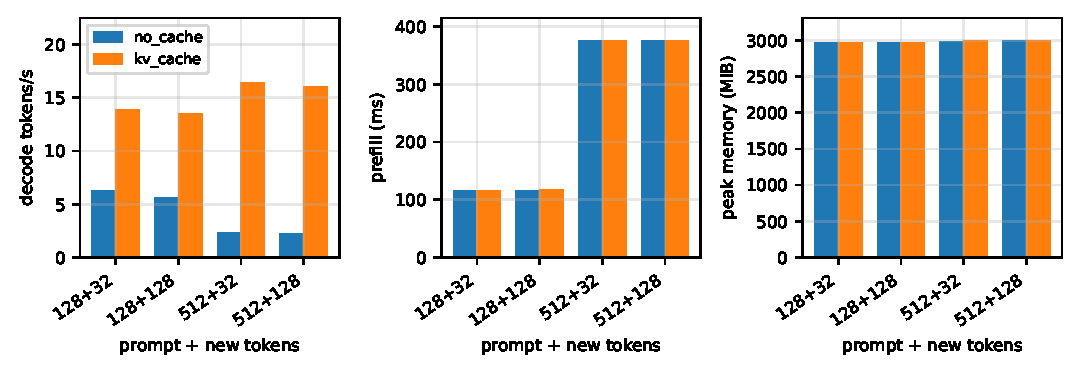
\includegraphics[width=\columnwidth]{kv_benchmark}
\caption{Decode throughput, prefill time and peak memory of the uncached and cached decoders for four prompt+new-token settings. The cache removes the dependence of decode speed on prompt length and does not change prefill time or peak memory noticeably.}
\label{fig:kv}
\end{figure}

\subsection{Tiled Online-Softmax Attention}
\label{sec:attres}
Table~\ref{tab:att} reports the maximum and mean absolute error of the reference, tiled and PyTorch fused implementations against an independent float64 reference over ten test cases: eight float32 cases (including a 5$\times$5 hand-checkable case with uneven tiles, non-divisible lengths such as 100 and 257, non-causal attention, a single query attending to 129 cached keys, a 16-query chunk attending to 144 keys, and scores in the hundreds to test the stable softmax), one fp16 and one bf16 case. In float32 all three implementations agree with the float64 result to within $10^{-4}$ (tiled: max $4.2\times10^{-5}$, mean $4.0\times10^{-8}$), no output contains NaN, and in fp16/bf16 the errors are those of the storage format and not of the algorithm; the tiled version is as accurate as the fused backend. This supports the claim of Section~\ref{sec:attmethod} that online softmax is exact.

\begin{table}[t]
\caption{Absolute error versus a float64 reference (max over cases / mean of case means). Eight float32 cases, one fp16, one bf16; causal masks except one non-causal float32 case.}
\label{tab:att}
\centering\footnotesize
\begin{tabular}{llrr}
\hline
Precision & Implementation & Max abs.\ error & Mean abs.\ error \\
\hline
float32 & reference & $3.3\times10^{-5}$ & $4.2\times10^{-8}$ \\
float32 & tiled online softmax & $4.2\times10^{-5}$ & $4.0\times10^{-8}$ \\
float32 & PyTorch SDPA & $9.4\times10^{-5}$ & $1.3\times10^{-7}$ \\
float16 & tiled online softmax & $7.8\times10^{-4}$ & $3.3\times10^{-5}$ \\
float16 & PyTorch SDPA & $7.8\times10^{-4}$ & $4.5\times10^{-5}$ \\
bfloat16 & tiled online softmax & $7.6\times10^{-3}$ & $2.6\times10^{-4}$ \\
bfloat16 & PyTorch SDPA & $7.6\times10^{-3}$ & $3.6\times10^{-4}$ \\
\hline
\end{tabular}
\end{table}

Fig.~\ref{fig:att} gives the honest performance picture (fp16, 12 heads of size 64, causal, RTX~4050). \emph{Memory:} the reference implementation materialises the $L\times L$ score matrix and its extra memory grows quadratically from 4.5\,MiB at $L=256$ to 1152\,MiB at $L=4096$, whereas the tiled version needs only 7\,MiB (tile 64) or 20\,MiB (tile 256), a 59--158$\times$ reduction at $L=4096$ (the tiled memory grows only linearly, through the output and accumulators). \emph{Speed:} the educational implementation is \emph{slower} than the dense reference, by 34$\times$ for 64$\times$64 tiles (2463\,ms versus 72\,ms at $L=4096$) and 2$\times$ for 256$\times$256 tiles (148\,ms); compared with PyTorch's fused SDPA kernel (8.1\,ms at $L=4096$) they are 303$\times$ (tile 64) and 18$\times$ (tile 256) slower. The reason is that FlashAttention gains speed by keeping tiles in on-chip SRAM inside one fused kernel; our PyTorch loop launches several small kernels per tile, re-reads $Q$, $K$ and $V$ from global memory, and pays Python overhead, so with 64$\times$64 tiles at $L=4096$ it runs roughly 2000 tile iterations, each launching on the order of a dozen small kernels (our estimate; we did not count launches). The tiling therefore demonstrates the memory-saving algorithm and its exactness but not its speed benefit, which requires a fused kernel.

\begin{figure}[t]
\centering
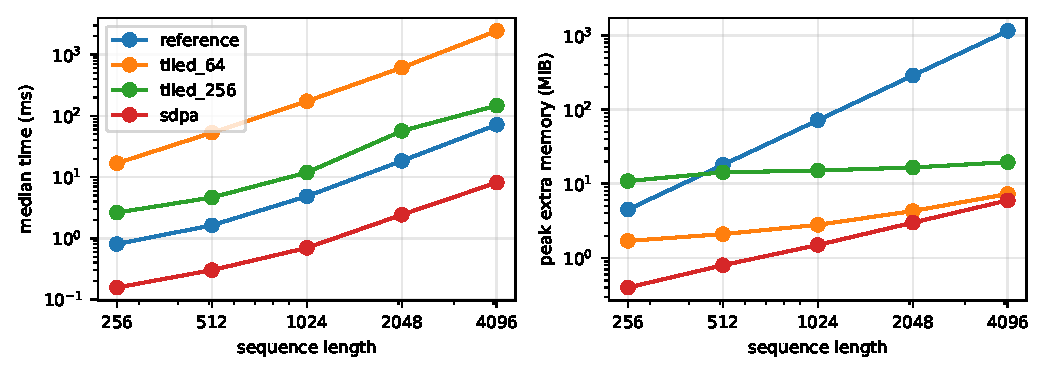
\includegraphics[width=\columnwidth]{attention_benchmark}
\caption{Median runtime (left) and peak extra GPU memory (right) of the four attention implementations versus sequence length (log--log, fp16). Tiled attention removes the quadratic memory growth of the reference but is slower in plain PyTorch than both the reference and the fused SDPA kernel.}
\label{fig:att}
\end{figure}

\subsection{Speculative Decoding}
\label{sec:specres}
\textbf{Correctness.} With the fine-tuned 1.5\,B target and the fine-tuned 0.5\,B draft (same tokenizer), the speculative decoder of Section~\ref{sec:specmethod} produced exactly the same tokens as plain cached greedy decoding for all 12 task prompts at every tested draft length $k\in\{2,4,6,8\}$, for 4 of 4 free-generation prompts (128 tokens, $k\in\{2,4,8\}$), and also matched Hugging Face's built-in assisted generation on 6 of 6 prompts. No fp16 divergence occurred in these runs, but it cannot be excluded in general because a $(k+1)$-token verification pass is numerically different from single-token steps (Section~\ref{sec:kvres}).

\textbf{Efficiency.} Table~\ref{tab:spec} and Fig.~\ref{fig:spec} show that the draft is highly accurate for this task: 95\,\% of proposed tokens are accepted at $k=2$ and 90\,\% at $k=4$, giving up to 7.2 tokens per target forward pass at $k=8$. Yet speculative decoding is \emph{slower} than plain cached decoding in every configuration: 0.71--0.80$\times$ on the task answers (best $k=4$: 8.74 versus 10.97 tokens/s) and 0.72--0.82$\times$ on long free generation (best $k=4$: 11.25 versus 13.81 tokens/s). Both models are resident in every run (about 3.9\,GB peak); speculative decoding adds 29--92\,MiB of peak memory for the draft cache and verification activations (4037 versus 3945\,MiB on the task answers, 3949 versus 3920\,MiB on free generation). Longer drafts reduce the acceptance rate (0.78 at $k=8$ for task answers, 0.62 for free text), so the benefit saturates early.

\begin{table*}[t]
\caption{Speculative decoding (fine-tuned 1.5B target, fine-tuned 0.5B draft, fp16, greedy) versus plain KV-cached greedy decoding. Task answers: 12 validation prompts, stop at EOS, at most 48 tokens (193 tokens in total); free generation: 4 prompts $\times$ 128 tokens. ``Tok./target fwd'' is accepted draft tokens plus one per round. Output was token-identical to greedy in all rows.}
\label{tab:spec}
\centering\footnotesize
\begin{tabular}{lrrrrrrr}
\hline
Workload & Method & Seconds & Tokens/s & Speed-up & Acceptance & Tok./target fwd & Peak MiB \\
\hline
Task answers & greedy KV & 17.6 & 10.97 & 1.00 & -- & 1.00 & 3945 \\
Task answers & spec.\ $k=2$ & 22.6 & 8.56 & 0.78 & 0.949 & 2.90 & 4037 \\
Task answers & spec.\ $k=4$ & 22.1 & 8.74 & 0.80 & 0.897 & 4.59 & 4037 \\
Task answers & spec.\ $k=6$ & 23.3 & 8.27 & 0.75 & 0.901 & 6.41 & 4037 \\
Task answers & spec.\ $k=8$ & 24.7 & 7.82 & 0.71 & 0.780 & 7.24 & 4037 \\
Free generation & greedy KV & 37.1 & 13.81 & 1.00 & -- & 1.00 & 3920 \\
Free generation & spec.\ $k=2$ & 49.8 & 10.29 & 0.75 & 0.844 & 2.69 & 3949 \\
Free generation & spec.\ $k=4$ & 45.5 & 11.25 & 0.82 & 0.810 & 4.16 & 3949 \\
Free generation & spec.\ $k=8$ & 51.3 & 9.98 & 0.72 & 0.618 & 5.86 & 3949 \\
\hline
\end{tabular}
\end{table*}

\begin{figure}[t]
\centering
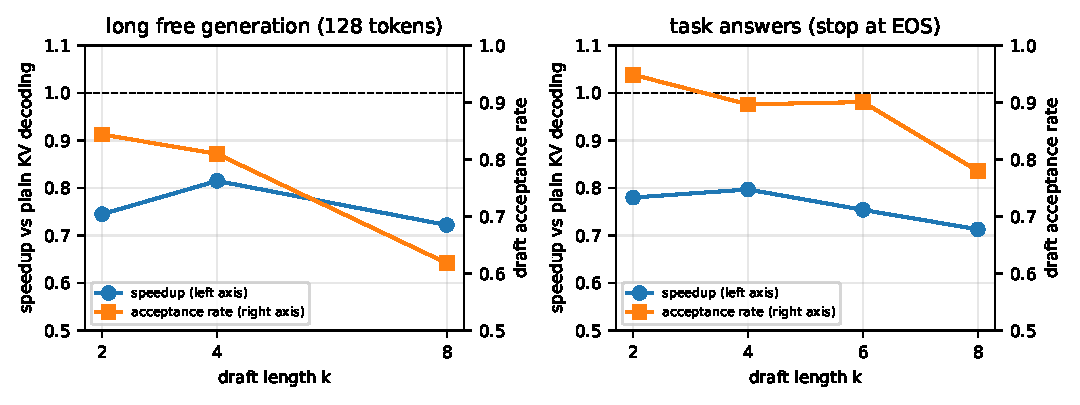
\includegraphics[width=\columnwidth]{spec_benchmark}
\caption{Speed-up over plain KV-cached decoding (blue, left axis) and draft acceptance rate (orange, right axis) versus draft length $k$ for the two workloads. Speed-up stays below the break-even line (dashed) although acceptance is high.}
\label{fig:spec}
\end{figure}

\textbf{Effect of fine-tuning the draft.} To check that adapting the draft was worthwhile, we repeated the task-answer benchmark with the \emph{untuned} Qwen2.5-0.5B-Instruct as draft (Table~\ref{tab:draftcmp}). The output of the target is again identical to greedy decoding for all 12 prompts and all $k$, which shows that correctness depends only on the verification step and not on the draft's quality. The fine-tuned draft, however, is accepted much more often (0.90 versus 0.62 at $k=4$) and gives 23--46\,\% more tokens per second than the untuned one (for example 8.74 versus 6.45 tokens/s at $k=4$), so the draft's training on the task is what keeps the slowdown moderate; with the untuned draft, speculative decoding runs at only 0.49--0.63$\times$ the speed of plain decoding.

\begin{table}[t]
\caption{Fine-tuned versus untuned 0.5B draft on the task answers (same target and prompts as Table~\ref{tab:spec}). Both variants reproduce the greedy output exactly (12 of 12 prompts).}
\label{tab:draftcmp}
\centering\footnotesize
\begin{tabular}{rcccccc}
\hline
 & \multicolumn{3}{c}{Fine-tuned draft} & \multicolumn{3}{c}{Untuned draft} \\
$k$ & Accept. & Tok./fwd & Speed-up & Accept. & Tok./fwd & Speed-up \\
\hline
2 & 0.949 & 2.90 & 0.78 & 0.667 & 2.33 & 0.63 \\
4 & 0.897 & 4.59 & 0.80 & 0.623 & 3.49 & 0.59 \\
6 & 0.901 & 6.41 & 0.75 & 0.644 & 4.87 & 0.57 \\
8 & 0.780 & 7.24 & 0.71 & 0.483 & 4.87 & 0.49 \\
\hline
\end{tabular}
\end{table}

\textbf{Why the slowdown.} A speculative round costs $k\,t_d + t_v$ (draft steps plus one verification pass) and yields $\bar n$ tokens, so the speed-up is $\bar n\,t_t/(k\,t_d+t_v)$ where $t_t$ is the target's one-token time. Table~\ref{tab:stepcost} gives the measured step times. The 0.5\,B draft needs 57\,ms per token against 71\,ms for the 1.5\,B target, a cost ratio $c=0.81$ and not the $c\ll1$ that speculative decoding assumes: both models run eagerly with a similar number of layers (24 versus 28) on a GPU where per-layer kernel-launch overhead, not arithmetic or memory bandwidth, dominates, so shrinking the model by 3$\times$ barely shortens a step. Conversely verifying $k+1$ tokens costs about the same as one token (68--75\,ms), which is why acceptance and tokens per round are good. Inserting the measured values predicts a speed-up of 0.96--1.13$\times$, still above the observed 0.71--0.80$\times$. We attribute the remaining gap to costs outside the timed forward passes: the draft model must also prefill the prompt (the task answers average only 16 tokens, so the extra prefill is a large share of the total), and our loop adds host--device synchronisation (one \texttt{.item()} per round), cache cropping and small tensor creations; we did not isolate these contributions individually. Speculative decoding would be expected to pay off with a much cheaper draft, a compiled or CUDA-graph decode loop, or a larger, more memory-bound target; we did not try these within the 6\,GB budget.

\begin{table}[t]
\caption{Measured step times (median of 15, prompt 256, KV cache) and predicted versus measured speed-up on the task answers. $c$ = draft / target one-token time.}
\label{tab:stepcost}
\centering\footnotesize
\begin{tabular}{rrrrrrr}
\hline
$k$ & Target 1-tok ms & Verify ($k+1$) ms & Draft 1-tok ms & $c$ & Predicted & Measured \\
\hline
2 & 71.1 & 68.0 & 57.4 & 0.81 & 1.13 & 0.78 \\
4 & 71.1 & 69.7 & 57.4 & 0.81 & 1.09 & 0.80 \\
6 & 71.1 & 74.6 & 57.4 & 0.81 & 1.09 & 0.75 \\
8 & 71.1 & 75.4 & 57.4 & 0.81 & 0.96 & 0.71 \\
\hline
\end{tabular}
\end{table}

\subsection{Application}
Figure~\ref{fig:app} shows the browser interface (Gradio, started with \texttt{python app/app.py}; models load on the first run, in about 13\,s). The user enters a patient note, inclusion and exclusion criteria, chooses the inference mode (no cache, KV cache, speculative with draft length $k$) and runs the screening. Figure~\ref{fig:report} shows the exported report for the built-in example: for each criterion it lists the decision, the cited sentence IDs with their exact text, a template explanation that quotes only those sentences, the rule-based overall outcome, the patient note as screened, and the provenance (model, adapter, decoding mode), together with the educational-prototype disclaimer. For labels without a cited sentence the explanation states that the absence of evidence is not proof, as in the last row of the figure. A second tab runs the three decoders on the user's own input and reports time, tokens/s, peak memory and token equality (on the example: 5.1 versus 12.5 versus 8.8 tokens/s for no cache, KV cache and speculative decoding, all producing identical tokens); a third tab shows the saved benchmark tables. An automated test (\texttt{src/test\_app.py}, 18 checks) verifies that empty or too short notes, missing criteria, more than 30 criteria and overlong criteria are rejected with a message, that the three modes return identical decisions, that every cited evidence text is the exact note sentence, and that the report contains the disclaimer and provenance but no local file paths; the same request also succeeds through the web API.

\begin{figure}[t]
\centering
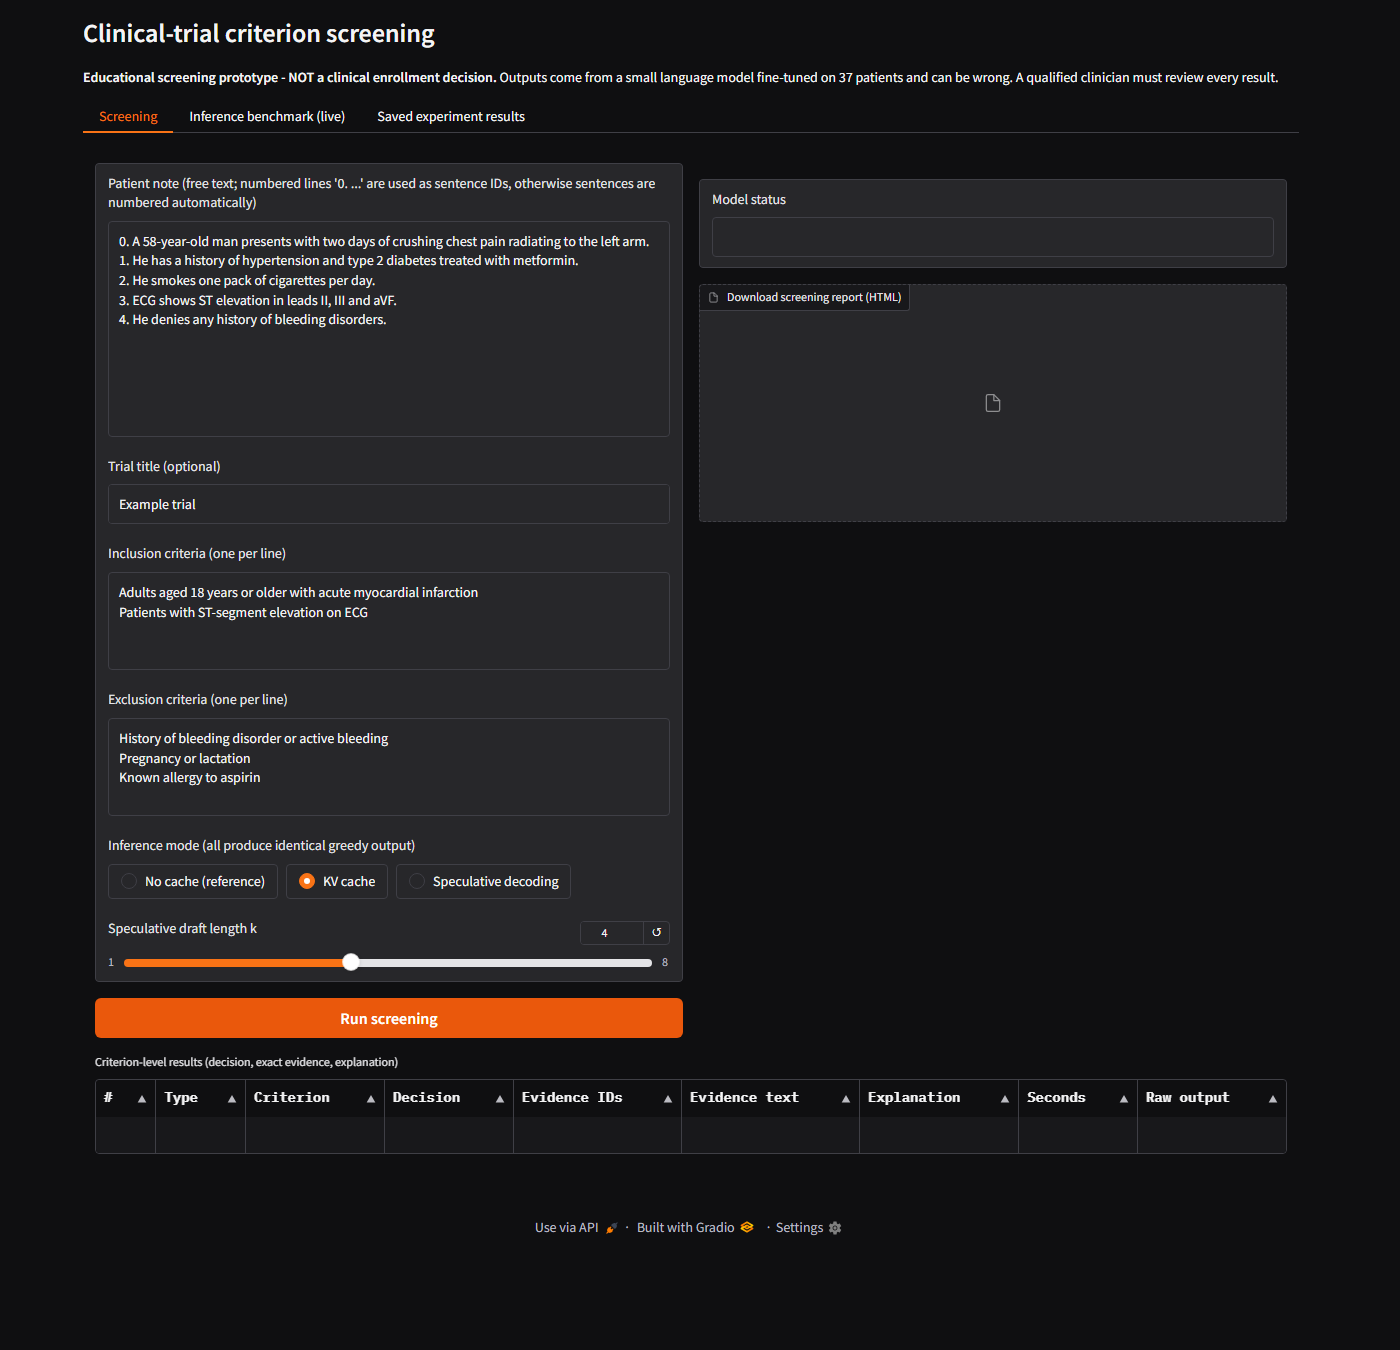
\includegraphics[width=\columnwidth]{app_screening}
\caption{Screenshot of the browser application: input of a patient note and criteria (left), inference mode and draft-length selection, model status and report download (right), and the criterion-level result table below.}
\label{fig:app}
\end{figure}

\begin{figure}[t]
\centering
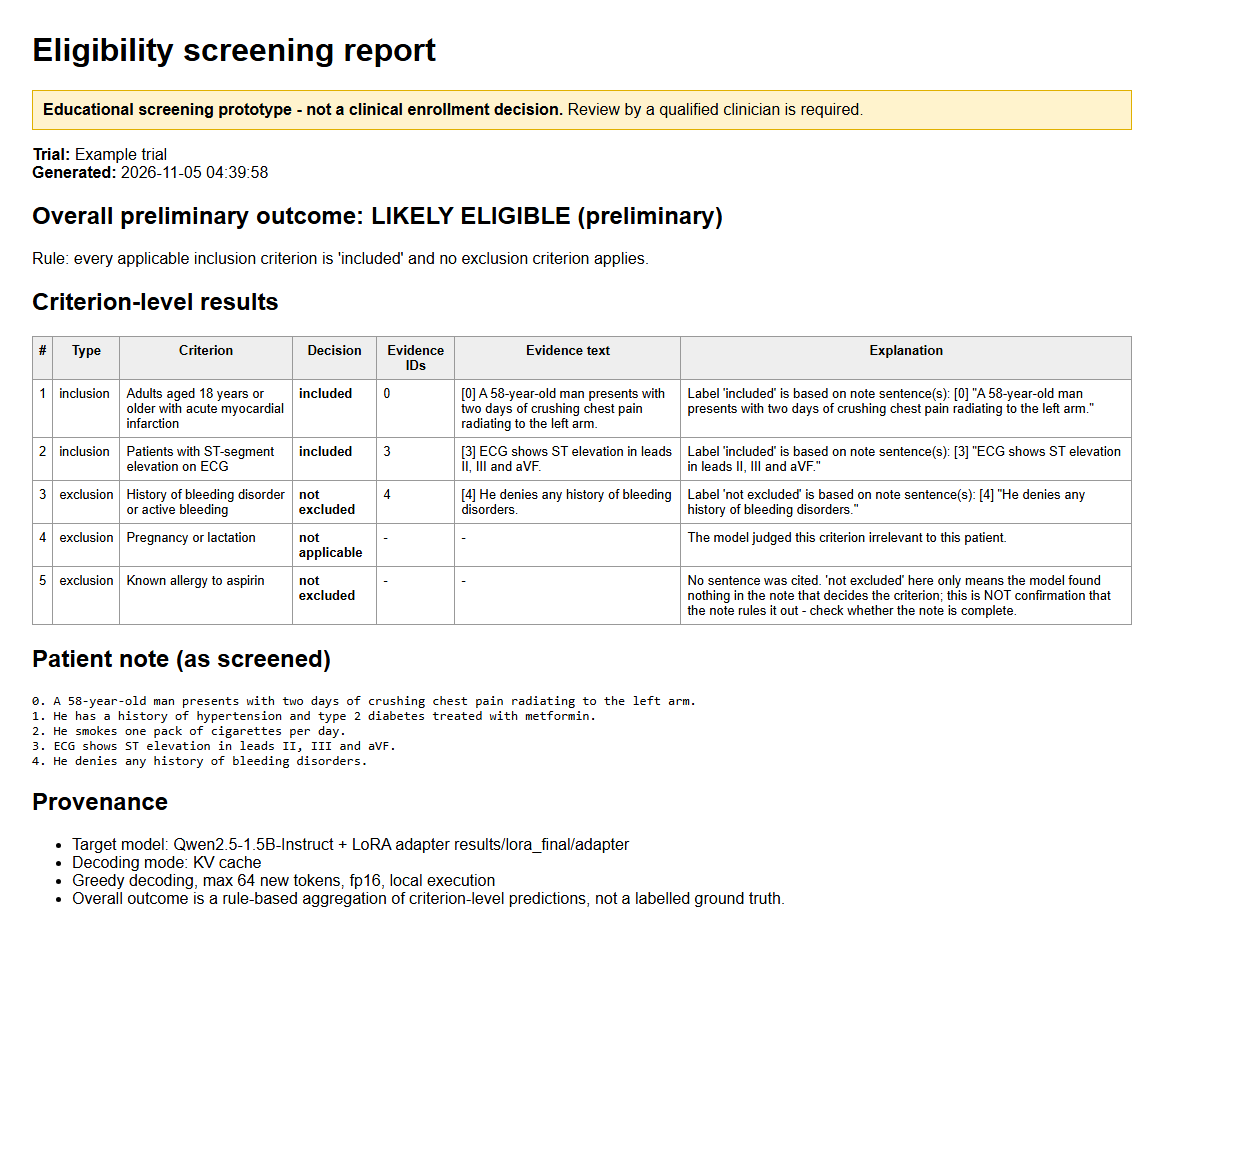
\includegraphics[width=\columnwidth]{app_report}
\caption{Exported screening report for the built-in example: criterion-level decisions with exact evidence, rule-based overall outcome, patient note and provenance, and the disclaimer. The unsupported \emph{not excluded} decision in the last row carries an explicit warning.}
\label{fig:report}
\end{figure}

\section{Limitations}
\textbf{Data and evaluation.} The benchmark consists of 53 patients and 1015 criteria; the fixed split leaves only eight test patients. The 95\,\% bootstrap intervals in Table~\ref{tab:main} are wide (e.g.\ accuracy 0.60--0.80), several classes have a handful of test examples (\emph{not included}: 7, inclusion N/A: 3) and the test split contains \emph{no} \emph{excluded} example, so the detection of excluded patients is not evaluated. The patients are short curated case descriptions (at most 14 sentences and 372 tokens), not full electronic health records, so no conclusion about long, messy notes can be drawn; for the same reason truncation never occurred, and the behaviour for notes beyond 555 tokens is untested.

\textbf{Modelling.} Only two training configurations were tried and each was trained once with a single seed, so differences of a few points between runs (e.g.\ 0.728 versus 0.733 accuracy) are within noise; the macro-F1 gain of the balanced run (0.467 to 0.534 on validation) rests on the exclusion classes, which have few validation examples. Other open models (Llama-3.2-1B, Gemma-2-2B) were rejected on resource and licensing grounds without being trained, so we make no claim that Qwen2.5-1.5B is the best choice, only that it fits the budget. The model returns a label and sentence IDs; the displayed explanation is a template that quotes the cited sentences and is not a free-text rationale, so it cannot explain \emph{why} the sentences support the label. The model is weakest exactly where a screening tool needs care: it labels most missing-information exclusion criteria \emph{not excluded} (3 of 28 NEI rows correct) and omits evidence in 42 of 58 wrong predictions. The trial-level outcome in the application is a transparent rule-based aggregation that we did not validate against any ground truth.

\textbf{Inference experiments.} All timings come from one laptop GPU, one software stack and small samples (12 task prompts, 4 long prompts, three repeats for the KV benchmark); they are indicative, not definitive. Fp16 decoding is not bit-reproducible between the cached and uncached paths, and the observed divergences are explained by exact logit ties (Section~\ref{sec:kvres}); an fp32 test was possible only for the 0.5\,B model. The tiled attention is a forward-pass educational implementation (no backward pass, no fused kernel) and is slower than the dense reference (Section~\ref{sec:attres}); we do not claim a speed benefit, only exactness and lower memory. Speculative decoding is implemented for greedy decoding only; its slowdown is specific to this hardware, an eager decoding loop and a draft that is only 19\,\% cheaper than the target, and part of the gap between predicted and measured speed-up is not isolated. The application was tested through scripted and API calls and screenshots, not with a formal usability study.

\textbf{Intended use.} The system is an educational prototype. It must not be used for enrolment or any clinical decision.

\section{Conclusion}
We built and evaluated a complete, locally executable pipeline for criterion-level clinical-trial eligibility matching on a 6\,GB GPU. LoRA fine-tuning of Qwen2.5-1.5B-Instruct on only 37 patients raised held-out accuracy from 0.058 to 0.718 and macro-F1 from 0.084 to 0.604 while returning cited sentence IDs (evidence micro-F1 0.531 overall, 0.636 on rows with expert evidence), and class-balanced oversampling was the decisive design choice for the exclusion classes. The honest picture has two sides: the model beats a majority baseline overall and on inclusion criteria, but on exclusion criteria it does not beat it in accuracy and it largely fails to say ``not enough information'', treating silence in the note as eligibility. Our hand-written decoding components behaved as theory predicts: the explicit KV cache is exact in fp32 and 2.2--7$\times$ faster in fp16 (with divergences traced to exact logit ties), tiled online-softmax attention matches a float64 reference to $4\times10^{-5}$ while cutting attention memory by up to 158$\times$ at the price of speed in plain PyTorch, and cache-synchronised greedy speculative decoding reproduces greedy output exactly with 62--95\,\% draft acceptance but is 0.7--0.8$\times$ as fast on this hardware because the draft is almost as costly per step as the target. Future work includes a larger and more balanced evaluation (cross-validation over patients), calibration of the NEI decision, a cheaper or compiled draft, and generating rationales with verifiable citations.


\section*{Reproducibility and Availability}
Source code, split manifest, scripts, benchmark logs and instructions: \url{https://github.com/Abdullah-NasirQureshi/genai-trialgpt-criterion-matching}. The LoRA adapters are distributed as a GitHub release asset of that repository. Demonstration video: [TODO(author): insert video link].

\section*{Acknowledgment}
The dataset and original system are by the TrialGPT authors~\cite{jin2024trialgpt}; models are from the Qwen team~\cite{qwen2024qwen25}.

\bibliographystyle{IEEEtran}
\bibliography{refs}

\appendix[Use of AI Assistants]
This work was carried out with the help of an AI coding assistant (Anthropic Claude, via Claude Code), which was used for: drafting and debugging the data preparation, training, evaluation, KV-cache, tiled-attention, speculative-decoding and application code; running experiments and collecting logs; and drafting the text of this report. The assistant's output was run and tested: split integrity assertions, metric hand-checks, cached versus uncached token equality, attention agreement with a float64 reference, and speculative versus greedy token equality are all automated checks in the repository. Reused libraries are PyTorch, Hugging Face Transformers/PEFT/Datasets and Gradio. The TrialGPT repository was consulted only as a reference; none of its predictions or results are used. The author is responsible for the complete submission and can explain and modify each component.
% TODO(author): review and edit this appendix so it reflects your own use of AI assistants accurately.


\end{document}
